\documentclass[12pt]{article}

\usepackage{answers}
\usepackage{setspace}
\usepackage{graphicx}
\usepackage{enumitem}
\usepackage{multicol}
\usepackage{mathrsfs}
\usepackage[margin=1in]{geometry} 
\usepackage{amsmath,amsthm,amssymb}
\usepackage{pgfplots}
\pgfplotsset{compat=1.15}
\usepackage{tikz-qtree}
\usepackage{color}
\usepackage{colortbl}
 
\newcommand{\N}{\mathbb{N}}
\newcommand{\Z}{\mathbb{Z}}
\newcommand{\C}{\mathbb{C}}
\newcommand{\R}{\mathbb{R}}

\DeclareMathOperator{\sech}{sech}
\DeclareMathOperator{\csch}{csch}
 
\newenvironment{theorem}[2][Theorem]{\begin{trivlist}
\item[\hskip \labelsep {\bfseries #1}\hskip \labelsep {\bfseries #2.}]}{\end{trivlist}}
\newenvironment{definition}[2][Definition]{\begin{trivlist}
\item[\hskip \labelsep {\bfseries #1}\hskip \labelsep {\bfseries #2.}]}{\end{trivlist}}
\newenvironment{proposition}[2][Proposition]{\begin{trivlist}
\item[\hskip \labelsep {\bfseries #1}\hskip \labelsep {\bfseries #2.}]}{\end{trivlist}}
\newenvironment{lemma}[2][Lemma]{\begin{trivlist}
\item[\hskip \labelsep {\bfseries #1}\hskip \labelsep {\bfseries #2.}]}{\end{trivlist}}
\newenvironment{exercise}[2][Exercise]{\begin{trivlist}
\item[\hskip \labelsep {\bfseries #1}\hskip \labelsep {\bfseries #2.}]}{\end{trivlist}}
\newenvironment{solution}[2][Solution]{\begin{trivlist}
\item[\hskip \labelsep {\bfseries #1}]}{\end{trivlist}}
\newenvironment{problem}[2][Problem]{\begin{trivlist}
\item[\hskip \labelsep {\bfseries #1}\hskip \labelsep {\bfseries #2.}]}{\end{trivlist}}
\newenvironment{question}[2][Question]{\begin{trivlist}
\item[\hskip \labelsep {\bfseries #1}\hskip \labelsep {\bfseries #2.}]}{\end{trivlist}}
\newenvironment{corollary}[2][Corollary]{\begin{trivlist}
\item[\hskip \labelsep {\bfseries #1}\hskip \labelsep {\bfseries #2.}]}{\end{trivlist}}
 
\begin{document}
 
% --------------------------------------------------------------
%                         Start here
% --------------------------------------------------------------
 
\title{Problem Set 2}%replace with the appropriate homework number
\author{Basil R. Yap\\ %replace with your name
40.316 Game Theory - Term 8} %if necessary, replace with your course title
 
\maketitle
%Below is an example of the problem environment

% Question 1
\begin{figure}[h!]
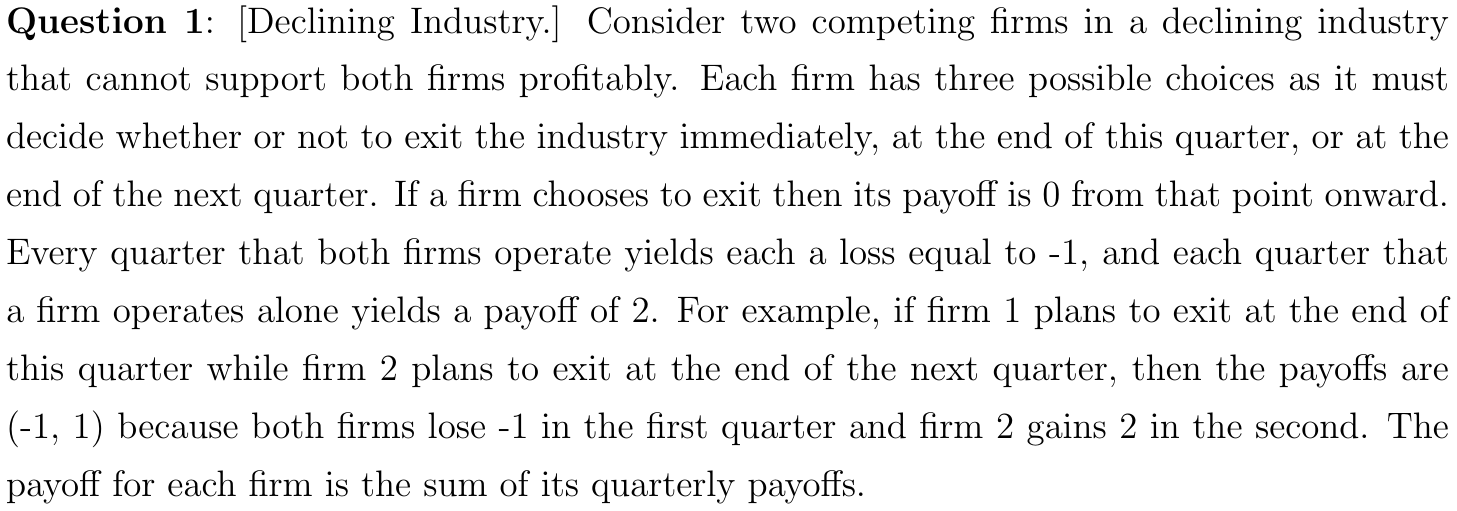
\includegraphics[width=\linewidth]{./assets/201806021724.png}
\end{figure}
\begin{enumerate}[label=(\alph*)]
\item Write down this game in matrix form
\item Is there any pure strategy that is dominated by some mixed strategy? Why?
\item Find the pure strategy Nash equilibria.
\item Find the unique mixed strategy Nash equilibrium (hint: you can use your answer to (b) to make things easier).
\end{enumerate}

\begin{solution}{}~\\
\begin{enumerate}[label=(\alph*)]
\item $$\begin{array}{rl}
A: & \text{Exit Immediately}\\
B: & \text{Exit at the end of this quarter}\\
C: & \text{Exit at the end of next quarter}
\end{array}$$
\begin{center}
\begin{tabular}{| c || c | c | c |}\hline
& A & B & C \\ \hline \hline
A & (0,0) & (0,2) & (0,4) \\ \hline
B & (2,0) & (-1,-1) & (-1,1) \\ \hline
C & (4,0) & (1,-1) & (-2,-2) \\ \hline
\end{tabular}
\end{center}
\item Pure Strategy $B$ is weakly dominated by a mixed strategy of $A$ and $C$.\\
This can be confirmed by comparing the expected pay-off, such that:
$$u_i([\frac{1}{2},0,\frac{1}{2}],s)\geq u_i(B,s)\ \ \ \ \forall i\in\{1,2\}\ \forall s\in\{A,B,C\}$$
\begin{align*}
u_1([\frac{1}{2},0,\frac{1}{2}],A)&\geq u_1(B,A)\\
\frac{1}{2}(0)+\frac{1}{2}(4)&\geq2\\
2&\geq2\text{ // True}\\
u_1([\frac{1}{2},0,\frac{1}{2}],B)&\geq u_1(B,B)\\
\frac{1}{2}(0)+\frac{1}{2}(1)&\geq-1\\
\frac{1}{2}&\geq-1\text{ // True}\\
u_1([\frac{1}{2},0,\frac{1}{2}],C)&\geq u_1(B,C)\\
\frac{1}{2}(0)+\frac{1}{2}(-2)&\geq-1\\
-1&\geq-1\text{ // True}
\end{align*}
Since the game is symmetrical, same applies for Column Player.
\item The Best Response for Row/Column Player:\\
\begin{align*}
BR_i(A) &= C\\
BR_i(B) &= C\\
BR_i(C) &= A
\end{align*}
\begin{center}
\begin{tikzpicture}
\begin{axis}[
axis lines=left,
xlabel = {$s_1$},
ylabel = {$s_2$},
xmin = 0,
xmax = 4,
ymin = 0,
ymax = 4,
xtick = {1,2,3},
xticklabels = {$A$,$B$,$C$},
ytick = {1,2,3},
yticklabels = {$A$,$B$,$C$}
]
\node[circle,fill,inner sep=2pt] at (axis cs:1, 3){};
\node[circle,fill,inner sep=2pt] at (axis cs:2, 3){};
\node[circle,fill,inner sep=2pt] at (axis cs:3, 1){};
\node[circle,draw,inner sep=3pt] at (axis cs:3, 1){};
\node[circle,draw,inner sep=3pt] at (axis cs:3, 2){};
\node[circle,draw,inner sep=3pt] at (axis cs:1, 3){};
\matrix [draw,below left] at (axis cs:4, 4) {
  \node [circle,draw,inner sep=3pt,label=right:$BR_1$] {}; \\
  \node [circle,fill,inner sep=2pt,label=right:$BR_2$] {}; \\
};
\end{axis}
\end{tikzpicture}
\end{center}
\begin{center}
$\therefore$ Pure Strategy Nash Equilibria at ($A,C$) and ($C,A$)
\end{center}
\item Based on the result in $(b)$, we only consider the strategies $A$ and $C$.\\
$$
\begin{array}{rl}
p: & \text{Probability row player chooses }A\text{ over C}\\
q: & \text{Probability column player chooses }A\text{ over C}
\end{array}
$$
Expected pay-off for row player given row player's action:\\

\begin{align*}
u_1(A,[q,1-q])&=0\\
u_1(C,[q,1-q])&=4q-2(1-q)\\
\text{Solve }u_1(A,[q^*,1-q^*])&=u_1(C,[q^*,1-q^*])\\
4q^*&=2(1-q^*)\\
6q^*&=2\\
q^*&=\frac{1}{3}
\end{align*}
Expected pay-off for column player given column player's action:\\

\begin{center}
The pay-off matrix is symmetrical.\\
$\therefore p^*=\frac{1}{3}$
\end{center}
\begin{center}
$\therefore$ Mixed Strategy Nash Equilibrium at [($\frac{1}{3},0,\frac{2}{3}$),($\frac{1}{3},0,\frac{2}{3}$)]
\end{center}
\end{enumerate}
\end{solution}
\pagebreak
% Question 2
\begin{figure}[h!]
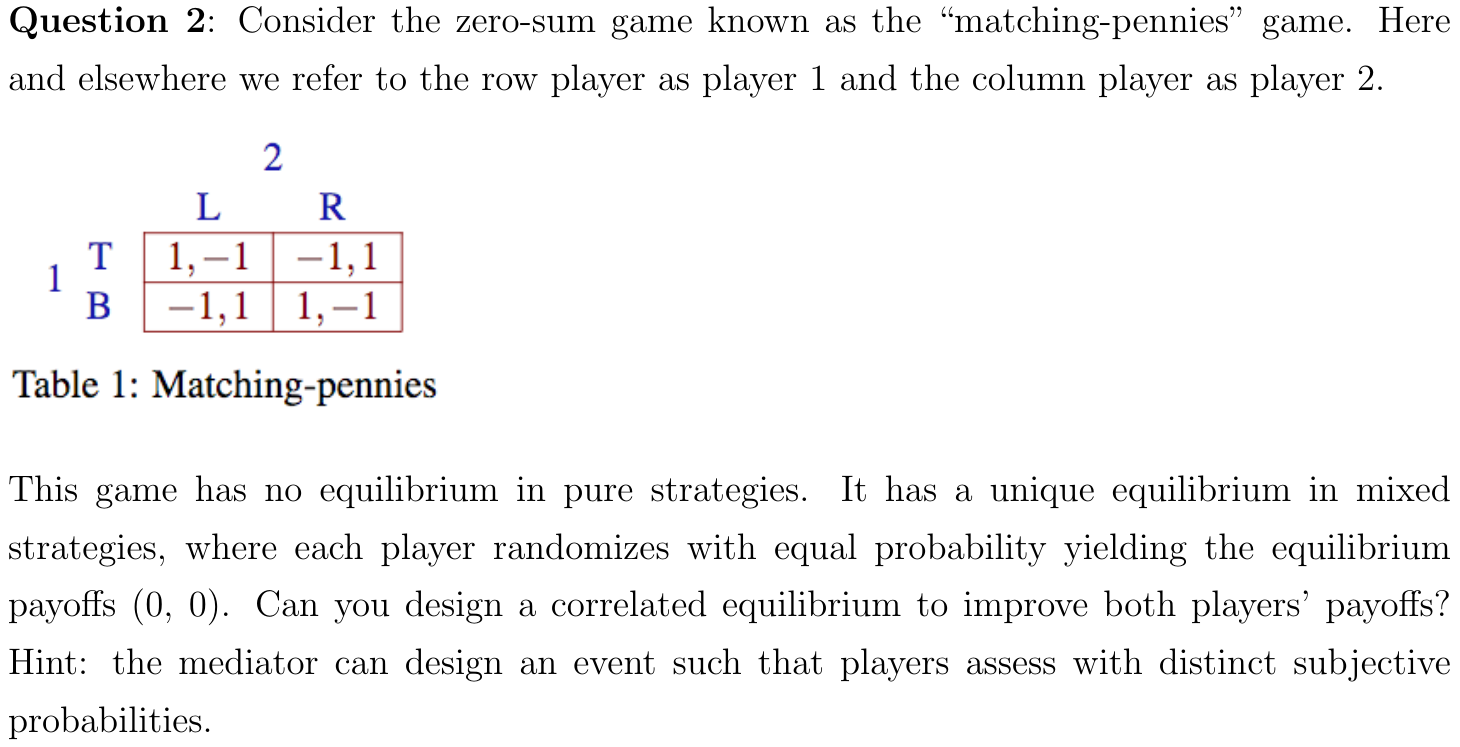
\includegraphics[width=\linewidth]{./assets/201806021725.png}
\end{figure}

\begin{solution}{}~\\

Consider the following states:\begin{enumerate}
\item[\textbf{State 1:}] where State 1 occurs when Event D is True,\\
Tell Player 1 to play T and Player 2 to play L.
\item[\textbf{State 2:}] where State 2 occurs when Event D is False,\\
Tell Player 1 to play B and Player 2 to play L.
\end{enumerate}
Where D has subjective probabilities,\\

$D=\left\{\begin{array}{ll}
\text{True} & \text{Where }\Pr(D;\text{Player 1})=p\text{ and }\Pr(D;\text{Player 2})=1-p\\
\text{False} & \text{Where }\Pr(D;\text{Player 1})=1-p\text{ and }\Pr(D;\text{Player 2})=p
\end{array}\right.$\\

The expected pay-off of both players are given by:
\begin{align*}
u_1(T|\text{ State 1})&=p(1)+(1-p)(-1)\\
&=2p-1\\
u_2(L|\text{ State 2})&=p(1)+(1-p)(-1)\\
&=2p-1
\end{align*}
\begin{center}
When $0.5\leq p<1$, the expected pay-off of both players are improved while the value of the game remains at 0. As the expected pay-off for both player has improved, neither will have incentive to deviate. Therefore, the solution is a correlated equilibrium.
\end{center}
\end{solution}
\pagebreak
% Question 3
\begin{figure}[h!]
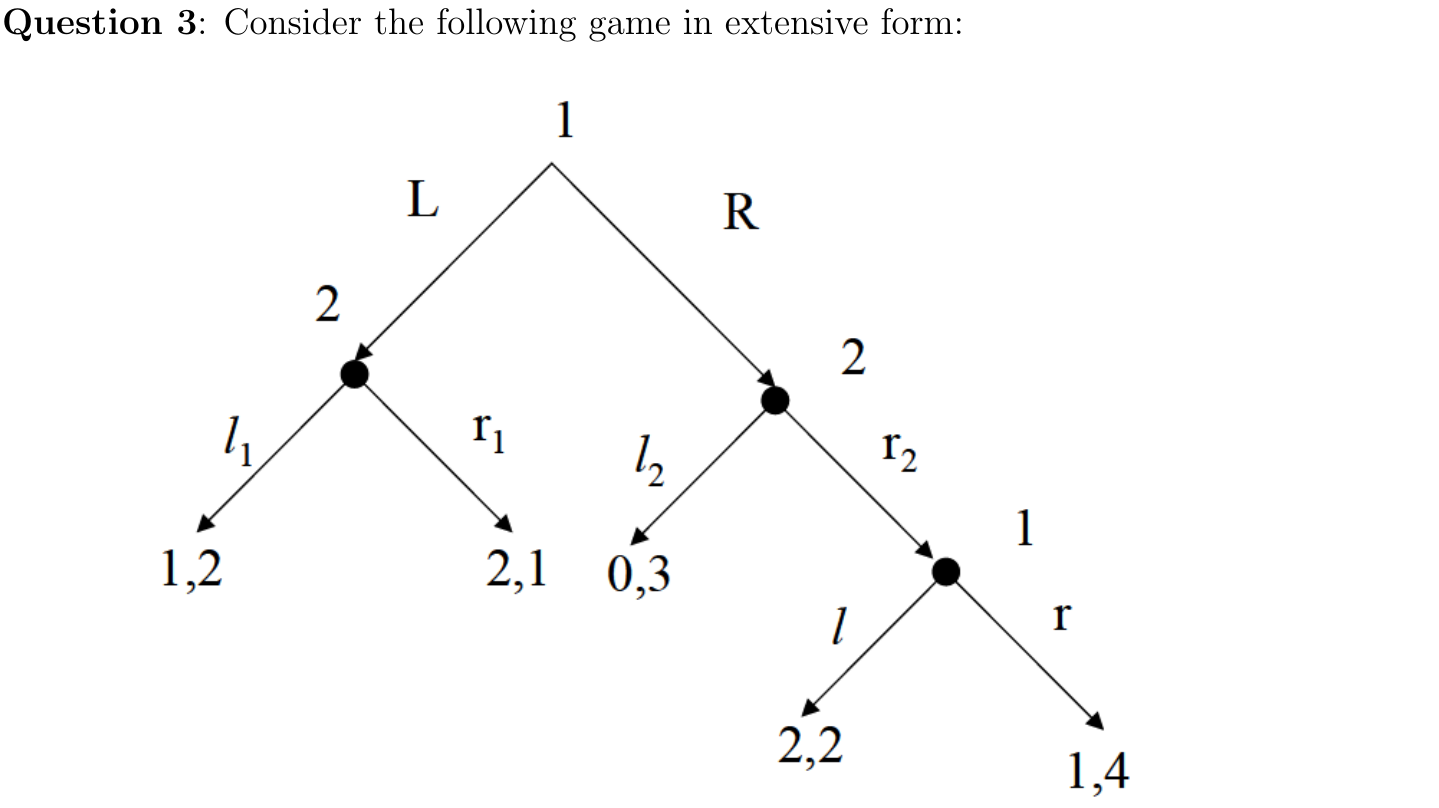
\includegraphics[width=\linewidth]{./assets/201806021726.png}
\end{figure}
\begin{enumerate}[label=(\alph*)]
\item Apply backwards induction in this game and find the subgame perfect equilibrium of the game
\item Write the game in normal-form and find the set of pure strategy Nash equilibria.
\end{enumerate}

\begin{solution}{}~\\
\begin{enumerate}[label=(\alph*)]
\item Using backwards induction:\\

\begin{center}
\begin{tikzpicture}[
	level distance=\linewidth/7,
	sibling distance=\linewidth/7,
	edge from parent path={(\tikzparentnode) -- (\tikzchildnode)}]
\Tree
[.\textbf{1}
    \edge node[auto=right,pos=.6] {L};
    [.\textbf{2} 
       \edge node[auto=right,pos=.6] {$l_1$};
       [.$(1,2)$ ]
       \edge node[auto=left,pos=.6] {$r_1$};
       [.$(2,1)$ ]
        ]
    \edge node[auto=left,pos=.6] {R};
    [.\textbf{2} 
        \edge node[auto=right,pos=.6] {$l_2$};
        [.$(0,3)$ ]
        \edge node[auto=left,pos=.6] {$r_2$};
        [.\textbf{1}
        		\edge node[auto=right,pos=.6] {$l$};
        		[.$(2,2)$ ]
        		\edge node[auto=left,pos=.6] {$r$};
        		[.$(1,4)$ ] 
        		]
        ]
]
\end{tikzpicture}\\
\begin{tikzpicture}[
	level distance=\linewidth/7,
	sibling distance=\linewidth/7,
	edge from parent path={(\tikzparentnode) -- (\tikzchildnode)}]
\Tree
[.\textbf{1}
    \edge node[auto=right,pos=.6] {L};
    [.2 
       \edge node[auto=right,pos=.6] {$l_1$};
       [.$(1,2)$ ]
       \edge node[auto=left,pos=.6] {$r_1$};
       [.$(2,1)$ ]
        ]
    \edge node[auto=left,pos=.6] {R};
    [.\textbf{2} 
        \edge node[auto=right,pos=.6] {$l_2$};
        [.$(0,3)$ ]
        \edge node[auto=left,pos=.6] {$r_2$};
        [.\textbf{1}
        		\edge node[auto=left,pos=.6] {$l$};
        		[.$(2,2)$ ]
        		]
        ]
]
\end{tikzpicture}\\
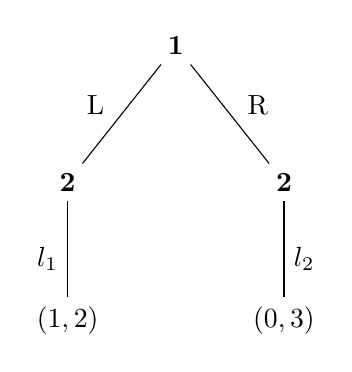
\begin{tikzpicture}[
	level distance=\linewidth/7,
	sibling distance=\linewidth/7,
	edge from parent path={(\tikzparentnode) -- (\tikzchildnode)}]
\Tree
[.\textbf{1}
    \edge node[auto=right,pos=.6] {L};
    [.\textbf{2} 
       \edge node[auto=right,pos=.6] {$l_1$};
       [.$(1,2)$ ]
        ]
    \edge node[auto=left,pos=.6] {R};
    [.\textbf{2} 
        \edge node[auto=left,pos=.6] {$l_2$};
        [.$(0,3)$ ]
        ]
]
\end{tikzpicture}\\
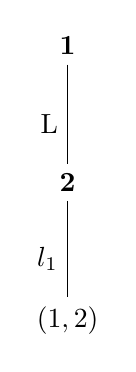
\begin{tikzpicture}[
	level distance=\linewidth/7,
	sibling distance=\linewidth/7,
	edge from parent path={(\tikzparentnode) -- (\tikzchildnode)}]
\Tree
[.\textbf{1}
    \edge node[auto=right,pos=.6] {L};
    [.\textbf{2} 
       \edge node[auto=right,pos=.6] {$l_1$};
       [.$(1,2)$ ]
        ]
]
\end{tikzpicture}\\
$\therefore$ The subgame perfect equilibrium is $(Ll,l_1l_2)$.
\end{center}
\item Normal-form pay-off matrix:\\

\begin{center}
\begin{tabular}{| c || c | c | c | c |}\hline
& $l_1l_2$ & $l_1r_2$ & $r_1l_2$ & $r_1r_2$\\ \hline\hline
$Ll$ & \cellcolor{blue!25}$\bold{(1,2)}$ & $(1,2)$ & $(2,1)$ & $(2,1)$ \\ \hline
$Lr$ & \cellcolor{blue!25}$\bold{(1,2)}$ & $(1,2)$ & $(2,1)$ & $(2,1)$ \\ \hline
$Rl$ & $(0,3)$ & $(2,2)$ & $(0,3)$ & $(2,2)$ \\ \hline
$Rr$ & $(0,3)$ & $(1,4)$ & $(0,3)$ & $(1,4)$ \\ \hline
\end{tabular}\\

$\therefore$ the pure strategy equilibria is ($Ll,l_1l_2$) and ($Lr,l_1l_2$)
\end{center}
\end{enumerate}
\end{solution}

% Question 4
\begin{figure}[h!]
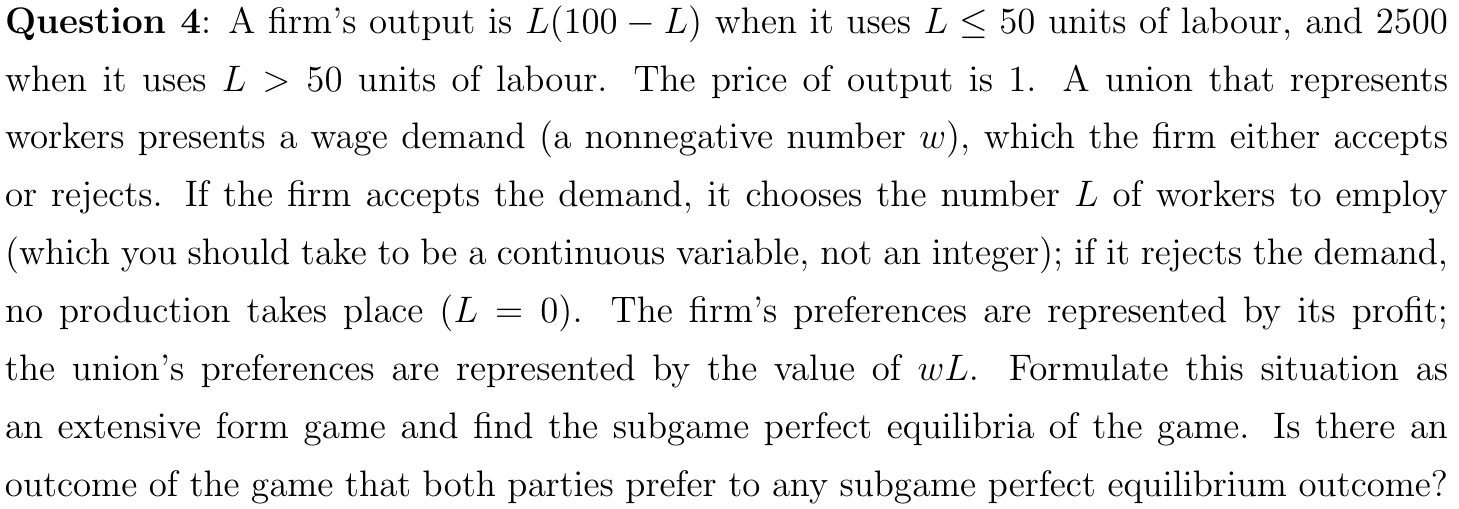
\includegraphics[width=\linewidth]{./assets/201806021727.png}
\end{figure}

\begin{solution}{}~\\
\begin{itemize}
\item Players: Firm (\textit{Player 1}), Union (\textit{Player 2})
\item Extensive form tree:\\

\begin{center}
\tikzset{
solid node/.style={circle,draw,inner sep=1.5,fill=black},
hollow node/.style={circle,draw,inner sep=1.5,fill=white}
}
\begin{tikzpicture}[scale=2]
\tikzstyle{level 1}=[level distance=10mm,sibling distance=5mm]
\tikzstyle{level 2}=[level distance=15mm,sibling distance=15mm]
\tikzstyle{level 3}=[level distance=10mm,sibling distance=5mm]
\tikzstyle{level 4}=[level distance=10mm,sibling distance=15mm]
\node(0)[solid node,label=above:{\textbf{2}}]{} 
	child{node(a1)[solid node, white,label=135:{$0$}]{}}
	child{[white] node(a2)[solid node, yshift=-9]{} 
		child{[black] node(b1)[hollow node,label=below:{$(0,0)$}]{} edge from parent node[left]{Reject $w$}}
		child{[black] node(b2)[solid node,label=45:{\textbf{1}}]{}
			child{node(c1)[solid node, white,label=135:{$0$}]{}}
			child{[white] node(c2)[solid node, yshift=-9]{}
				child{[black] node(d1)[hollow node,label=below:{$(u_1(L,w),u_2(L,w))$}]{}}
				edge from parent node[black, xshift=0,yshift=-0]{$L$}
				}
			child{node(c3)[solid node, white,label=45:{$\infty$}]{}}
		edge from parent node[right]{Accept $w$}}
 	edge from parent node[black, xshift=0,yshift=-20]{\textbf{1}}
 	edge from parent node[black, xshift=0,yshift=-0]{$w$}
	}
	child{node(a3)[solid node, white,label=45:{$\infty$}]{}};
\draw[dashed,bend right](a1)to(a3);
\draw[dashed,bend right](c1)to(c3);
\end{tikzpicture}
\end{center}
$$
u_1(L,w)=\left\{\begin{array}{ll}
L(100-L)-wL & L\leq50\\
2500-wL & L>50
\end{array}\right.
$$
$$
u_2(L,w)=wL
$$
\end{itemize}
\begin{center}
Row player does have increased pay-off when $L\leq50$, $\therefore$ consider $u_1$ only when $L\leq50$
\end{center}
\begin{align*}
u_1(L,w)&=L(100-L)-wL\\
&=100L-L^2-wL\\
\nabla u_1(L,w)&=\frac{d}{dL}(100L-L^2-wL)\\
&= 100-2L-w\\
\text{Solve }\nabla u_1(L^*,w)&= 0\\
100-2L^*-w &= 0\\
2L^*&=100-w\\
L^*&=\frac{1}{2}(100-w)
\end{align*}
\begin{center}
\tikzset{
solid node/.style={circle,draw,inner sep=1.5,fill=black},
hollow node/.style={circle,draw,inner sep=1.5,fill=white}
}
\begin{tikzpicture}[scale=2]
\tikzstyle{level 1}=[level distance=10mm,sibling distance=5mm]
\tikzstyle{level 2}=[level distance=15mm,sibling distance=15mm]
\tikzstyle{level 3}=[level distance=7mm,sibling distance=5mm]
\tikzstyle{level 4}=[level distance=10mm,sibling distance=15mm]
\node(0)[solid node,label=above:{\textbf{2}}]{} 
	child{node(a1)[solid node, white,label=135:{$0$}]{}}
	child{[white] node(a2)[solid node, yshift=-9]{} 
		child{[black] node(b1)[hollow node,label=below:{$(0,0)$}]{} edge from parent node[left]{Reject $w$}}
		child{[black] node(b2)[solid node,label=45:{\textbf{1}}]{}
			child{[black] node(c2)[solid node, yshift=-23]{}
				child{[black] node(d1)[hollow node,label=below:{$(u_1(L^*,w),u_2(L^*,w))$}]{}}
				edge from parent node[black, xshift=0,yshift=-28]{$L^*=\frac{1}{2}(100-w)$}
				}
		edge from parent node[right]{Accept $w$}}
 	edge from parent node[black, xshift=0,yshift=-20]{\textbf{1}}
 	edge from parent node[black, xshift=0,yshift=-0]{$w$}
	}
	child{node(a3)[solid node, white,label=45:{$\infty$}]{}};
\draw[dashed,bend right](a1)to(a3);
\end{tikzpicture}\\

Consider the cases where $u_1(L^*,w)<0$ and $u_1(L^*,w)>0$,\\
When $u_1(L^*,w)\leq0$, \textit{Player 1} would reject the $w$ proposed by \textit{Player 2}.\\
When $u_1(L^*,w)\geq0$, \textit{Player 1} would accept the $w$ proposed by \textit{Player 2}.
\end{center}
\begin{align*}
\text{Solve }u_1(L^*,w)&=0\\
100(\frac{1}{2}(100-w))-(\frac{1}{2}(100-w))^2-w(\frac{1}{2}(100-w))&=0\\
200(100-w)-(100-w)^2-2w(100-w)&=0\\
20000-200w-10000+200w-w^2-200w+2w^2&=0\\
w^2-200w+10000&=0\\
(w-100)^2&=0\\
w&=0
\end{align*}
\begin{center}
\tikzset{
solid node/.style={circle,draw,inner sep=1.5,fill=black},
hollow node/.style={circle,draw,inner sep=1.5,fill=white}
}
\begin{tikzpicture}[scale=2]
\tikzstyle{level 1}=[level distance=10mm,sibling distance=5mm]
\tikzstyle{level 2}=[level distance=15mm,sibling distance=15mm]
\tikzstyle{level 3}=[level distance=7mm,sibling distance=5mm]
\tikzstyle{level 4}=[level distance=10mm,sibling distance=15mm]
\node(0)[solid node,label=above:{\textbf{2}}]{} 
	child{node(a1)[solid node, white,label=135:{$100$}]{}}
	child{[white] node(a2)[solid node, yshift=-9]{} 
		child{[black] node(b1)[hollow node,label=below:{$(0,0)$}]{} edge from parent node[left]{Reject $w$, $w\geq100$}}
		child{[black] node(b2)[solid node,label=45:{\textbf{1}}]{}
			child{[black] node(c2)[solid node, yshift=-23]{}
				child{[black] node(d1)[hollow node,label=below:{$(u_1(L^*,w),u_2(L^*,w))$}]{}}
				edge from parent node[black, xshift=0,yshift=-28]{$L^*=\frac{1}{2}(100-w)$}
				}
		edge from parent node[right]{Accept $w$, $w\leq100$}}
 	edge from parent node[black, xshift=0,yshift=-20]{\textbf{1}}
 	edge from parent node[black, xshift=0,yshift=-0]{$w$}
	}
	child{node(a3)[solid node, white,label=45:{$\infty$}]{}};
\draw[dashed,bend right](a1)to(a3);
\end{tikzpicture}
\end{center}
\begin{center}
Consider the case when $w\leq100$ and $L=L^*$
\end{center}
\begin{align*}
u_2(L^*,w)&=\frac{1}{2}w(100-w)\\
\text{Solve }\nabla u_2(L^*,w*)&=0\\
\frac{d}{dw^*}(\frac{1}{2}w^*(100-w*))&=0\\
50-w*&=0\\
w^*&=50
\end{align*}
\begin{center}
\tikzset{
solid node/.style={circle,draw,inner sep=1.5,fill=black},
hollow node/.style={circle,draw,inner sep=1.5,fill=white}
}
\begin{tikzpicture}[scale=2]
\tikzstyle{level 1}=[level distance=15mm,sibling distance=25mm]
\tikzstyle{level 2}=[level distance=10mm,sibling distance=15mm]
\tikzstyle{level 3}=[level distance=10mm,sibling distance=15mm]
\tikzstyle{level 4}=[level distance=10mm,sibling distance=5mm]
\tikzstyle{level 5}=[level distance=10mm,sibling distance=15mm]
\node(0)[solid node,label=above:{\textbf{2}}]{}
	child{node(a1)[solid node,label=135:{\textbf{2}}]{}
		child{[black] node(c2)[solid node,label=left:{\textbf{1}}]{}
				child{[black] node(d2)[solid node,label=left:{\textbf{1}}]{}
					child{[black] node(e1)[hollow node, label=below:{$(u_1(L^*,w),u_2(L^*,w))$}]{}
							edge from parent node[left]{$L^*=\frac{1}{2}(100-w)$}						
						}
					edge from parent node[left]{Accept $w$}
					}
				edge from parent node[left]{$w=50$}			
			}
		child{[black] node(c3)[solid node,label=right:{\textbf{1}}]{}
				child{[black] node(d3)[solid node,label=right:{\textbf{1}}]{}
					child{[black] node(e2)[hollow node, label=below:{$(0,0)$}]{}
							edge from parent node[right]{$L^*=0$}						
						}
					edge from parent node[right]{Accept $w$}
					}
				edge from parent node[right]{$w=100$}			
			}
		edge from parent node[left]{$w\leq100$}
	}
	child{node(a2)[solid node,label=45:{\textbf{2}}, sibling distance=5mm]{} 
		child{node(b1)[solid node, white,label=135:{$100$}, xshift=50]{}	}
		child{[white] node(b2)[solid node, yshift=-11]{} 
			child{[black] node(c1)[hollow node,label=below:{$(0,0)$}]{}
					edge from parent node[right]{Reject $w$}				
				}
 			edge from parent node[black, xshift=0,yshift=-25]{\textbf{1}}
 			edge from parent node[black, xshift=0,yshift=-0]{$w$}		
			}
		child{node(b3)[solid node, white,label=45:{$\infty$}, xshift=-50]{}}
		edge from parent node[right]{$w\geq100$}
		};
\draw[dashed,bend right](b1)to(b3);
\end{tikzpicture}
\end{center}
\begin{center}
The subgame perfect equilibria are\\ $(Accept/L=25,w=50)$ , $(Accept/L=0,w=100)$\\
and $(Reject/L=0,w\in[100,\infty])$
\end{center}
\begin{center}
There is one subgame perfect equilibrium where both players benefit, that is at $(Accept/L=25,w=50)$.\\
The expected pay-off would be $(625,1250)$.
\end{center}
\end{solution}
\pagebreak
% Question 5
\begin{figure}[h!]

\includegraphics[width=\linewidth]{./assets/201806021728.png}
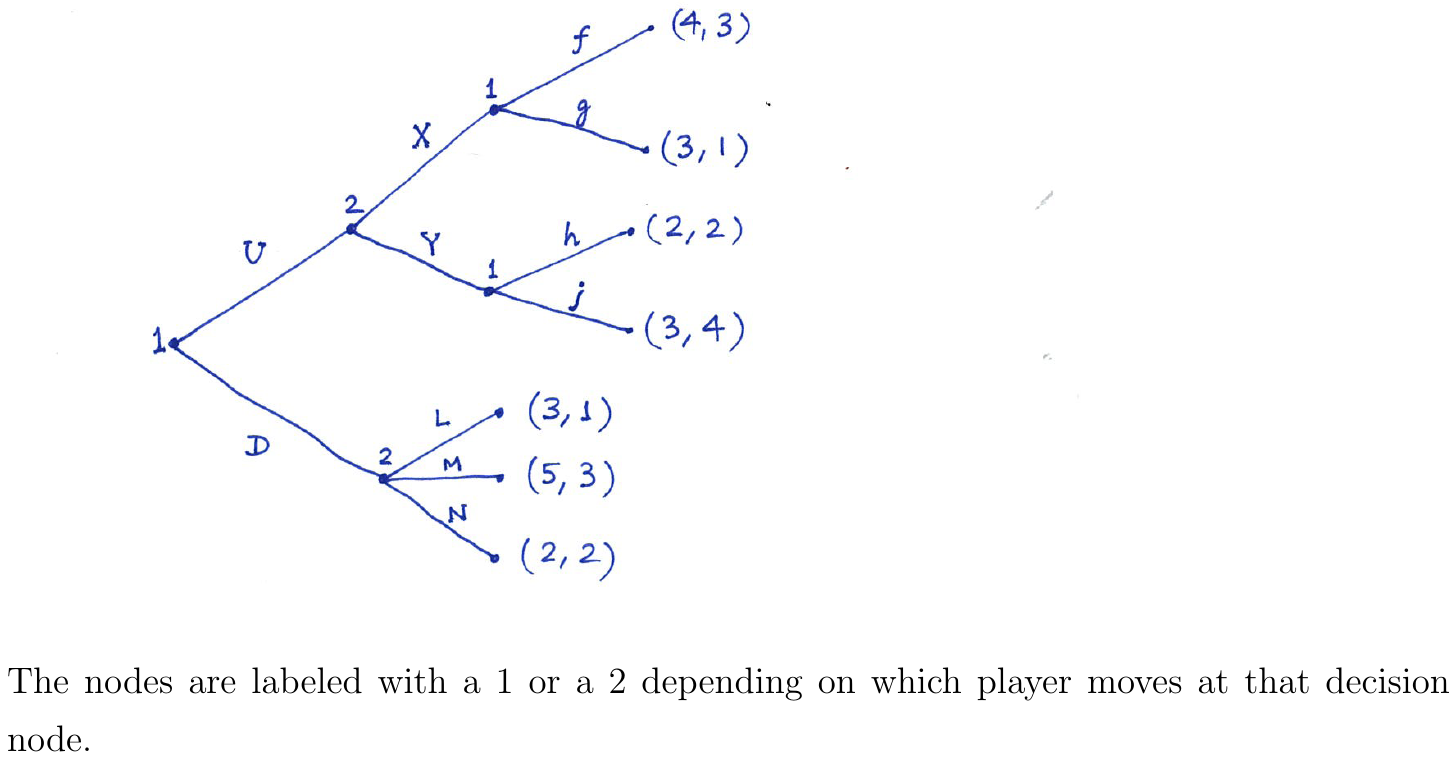
\includegraphics[width=\linewidth]{./assets/201806021729.png}
\end{figure}
\begin{enumerate}[label=(\alph*)]
\item Find a subgame perfect equilibrium (in pure strategies).
\item Is there a Nash equilibrium for the game that is not SPE? If yes, write down one such equilibrium.
\end{enumerate}

\begin{solution}{}~\\
\begin{enumerate}[label=(\alph*)]
\item Using backwards induction:\\

\begin{center}
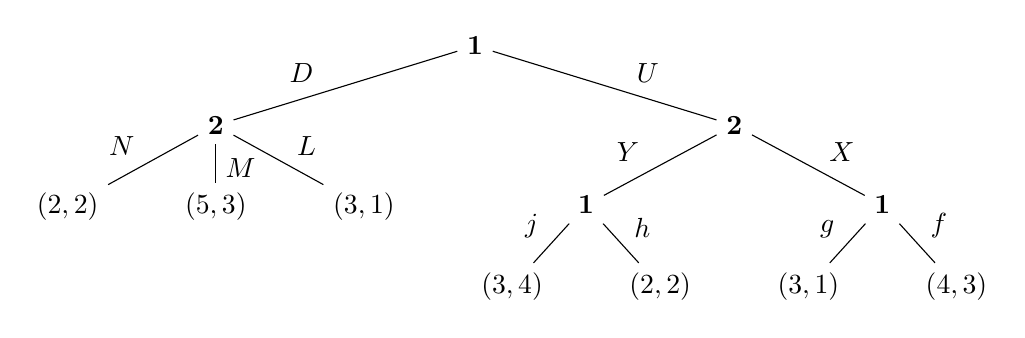
\begin{tikzpicture}[
	level distance=\linewidth/12,
	sibling distance=\linewidth/14,
	edge from parent path={(\tikzparentnode) -- (\tikzchildnode)}]
\Tree
[.\textbf{1}
    \edge node[auto=right,pos=.6] {$D$};
    [.\textbf{2} 
       \edge node[auto=right,pos=.6] {$N$};
       [.$(2,2)$ ]
       \edge node[auto=left,pos=.6] {$M$};
       [.$(5,3)$ ]
       \edge node[auto=left,pos=.6] {$L$};
       [.$(3,1)$ ]
    	]
    \edge node[auto=left,pos=.6] {$U$};
    [.\textbf{2} 
        \edge node[auto=right,pos=.6] {$Y$};
        [.\textbf{1} 
			\edge node[auto=right,pos=.6] {$j$};
			[.$(3,4)$ ]
			\edge node[auto=left,pos=.6] {$h$};
			[.$(2,2)$ ]        
        ]
        \edge node[auto=left,pos=.6] {$X$};
        [.\textbf{1}
        		\edge node[auto=right,pos=.6] {$g$};
        		[.$(3,1)$ ]
        		\edge node[auto=left,pos=.6] {$f$};
        		[.$(4,3)$ ] 
        		]
        ]
]
\end{tikzpicture}
\end{center}
\begin{center}
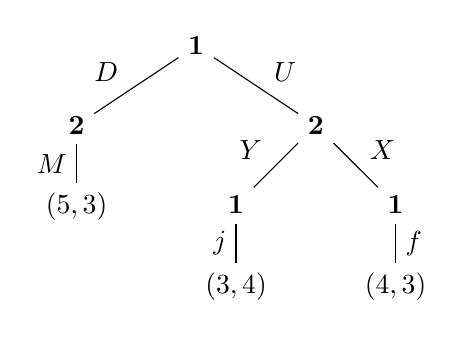
\begin{tikzpicture}[
	level distance=\linewidth/12,
	sibling distance=\linewidth/12,
	edge from parent path={(\tikzparentnode) -- (\tikzchildnode)}]
\Tree
[.\textbf{1}
    \edge node[auto=right,pos=.6] {$D$};
    [.\textbf{2}
       \edge node[auto=right] {$M$};
       [.$(5,3)$ ]
    	]
    \edge node[auto=left,pos=.6] {$U$};
    [.\textbf{2} 
        \edge node[auto=right,pos=.6] {$Y$};
        [.\textbf{1} 
			\edge node[auto=right] {$j$};
			[.$(3,4)$ ]        
        ]
        \edge node[auto=left,pos=.6] {$X$};
        [.\textbf{1}
        		\edge node[auto=left] {$f$};
        		[.$(4,3)$ ] 
        		]
        ]
]
\end{tikzpicture}
\end{center}
\begin{center}
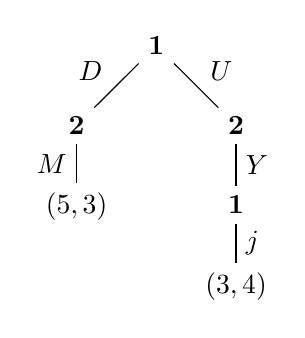
\begin{tikzpicture}[
	level distance=\linewidth/12,
	sibling distance=\linewidth/12,
	edge from parent path={(\tikzparentnode) -- (\tikzchildnode)}]
\Tree
[.\textbf{1}
    \edge node[auto=right,pos=.6] {$D$};
    [.\textbf{2}
       \edge node[auto=right] {$M$};
       [.$(5,3)$ ]
    	]
    \edge node[auto=left,pos=.6] {$U$};
    [.\textbf{2} 
        \edge node[auto=left] {$Y$};
        [.\textbf{1} 
			\edge node[auto=left] {$j$};
			[.$(3,4)$ ]        
        ]
    	]
]
\end{tikzpicture}
\end{center}
\begin{center}
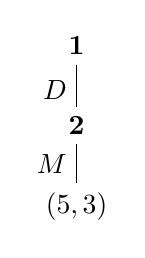
\begin{tikzpicture}[
	level distance=\linewidth/12,
	sibling distance=\linewidth/12,
	edge from parent path={(\tikzparentnode) -- (\tikzchildnode)}]
\Tree
[.\textbf{1}
    \edge node[auto=right,pos=.6] {$D$};
    [.\textbf{2}
       \edge node[auto=right] {$M$};
       [.$(5,3)$ ]
    	]
]
\end{tikzpicture}
\end{center}
\begin{center}
The subgame perfect equilibrium exists at $(Djf,MY)$
\end{center}
\item Normal-form pay-off matrix:\\

\begin{center}
\begin{tabular}{| c || c | c | c | c | c | c |}\hline
& $NY$ & $NX$ & $MY$ & $MX$ & $LY$ & $LX$ \\ \hline\hline
$Djg$ & $(2,2)$ & $(2,2)$ & \cellcolor{blue!25}$\bold{(5,3)}$ & \cellcolor{blue!25}$\bold{(5,3)}$ & $(3,1)$ & $(3,1)$ \\ \hline
$Djf$ & $(2,2)$ & $(2,2)$ & \cellcolor{blue!25}$\bold{(5,3)}$ & \cellcolor{blue!25}$\bold{(5,3)}$ & $(3,1)$ & $(3,1)$ \\ \hline
$Dhg$ & $(2,2)$ & $(2,2)$ & \cellcolor{blue!25}$\bold{(5,3)}$ & \cellcolor{blue!25}$\bold{(5,3)}$ & $(3,1)$ & $(3,1)$ \\ \hline
$Dhf$ & $(2,2)$ & $(2,2)$ & \cellcolor{blue!25}$\bold{(5,3)}$ & \cellcolor{blue!25}$\bold{(5,3)}$ & $(3,1)$ & $(3,1)$ \\ \hline
$Ujg$ & \cellcolor{blue!25}$\bold{(3,4)}$ & $(3,1)$ & $(3,4)$ & $(3,1)$ & \cellcolor{blue!25}$\bold{(3,4)}$ & $(3,1)$ \\ \hline
$Ujf$ & \cellcolor{blue!25}$\bold{(3,4)}$ & $(4,2)$ & $(3,4)$ & $(4,2)$ & \cellcolor{blue!25}$\bold{(3,4)}$ & $(4,2)$ \\ \hline
$Uhg$ & $(2,2)$ & $(3,1)$ & $(2,2)$ & $(3,1)$ & $(2,2)$ & $(3,1)$ \\ \hline
$Uhf$ & $(2,2)$ & \cellcolor{blue!25}$\bold{(4,2)}$ & $(2,2)$ & $(4,2)$ & $(2,2)$ & \cellcolor{blue!25}$\bold{(4,2)}$ \\ \hline
\end{tabular}
\end{center}
\begin{center}
An example of a pure strategy Nash Equilibrium\\
which is not a sub-game perfect equilibrium is $(Ujg,NY)$.
\end{center}
\end{enumerate}
\end{solution}

% Question 5
\begin{figure}[h!]
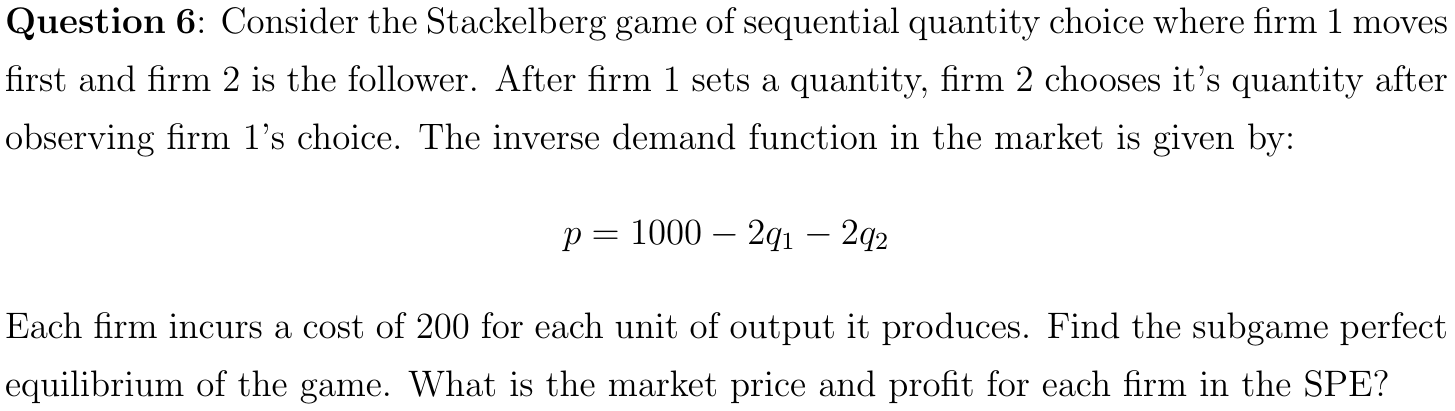
\includegraphics[width=\linewidth]{./assets/201806021730.png}
\end{figure}

\begin{solution}{}~\\
\begin{center}
\tikzset{
solid node/.style={circle,draw,inner sep=1.5,fill=black},
hollow node/.style={circle,draw,inner sep=1.5,fill=white}
}
\begin{tikzpicture}[scale=4]
\tikzstyle{level 1}=[level distance=7mm,sibling distance=5mm]
\tikzstyle{level 2}=[level distance=7mm,sibling distance=5mm]
\node(0)[solid node,label=above:{\textbf{1}}]{} 
	child{node(a1)[solid node, white,label=135:{$0$}]{}}
	child{[white] node(a2)[solid node, yshift=-17]{}
		child{[black] node(b1)[solid node, white,label=135:{$0$}]{}
		}
			child{[white] node(b2)[hollow node,black,fill=white,yshift=-17]{}
 				edge from parent node[black]{$q_2$}
 				edge from parent node[black,yshift=-70]{$(u_1(q_1,q_2),u_2(q_1,q_2))$}
			}
		child{[black] node(b3)[solid node, white,label=45:{$\infty$}]{}}
 		edge from parent node[black, xshift=0,yshift=-45]{\textbf{2}}
 		edge from parent node[black, xshift=0,yshift=-0]{$q_1$}
	}
	child{node(a3)[solid node, white,label=45:{$\infty$}]{}};
\draw[dashed,bend right](a1)to(a3);
\draw[dashed,bend right](b1)to(b3);
\end{tikzpicture}
\end{center}
\begin{align*}
u_1(q_1,q_2)&=q_1(1000-2q_1-2q_2)-200q_1\\
u_2(q_1,q_2)&=q_2(1000-2q_1-2q_2)-200q_2
\end{align*}
\begin{align*}
\nabla u_2(q_1,q_2)&=\frac{d}{dq_2}\left(q_2(1000-2q_1-2q_2)-200q_2\right)\\
&=1000-2q_1-4q_2-200\\
&=800-2q_1-4q_2
\end{align*}\\
\begin{align*}
\text{Solve }\nabla u_2(q_1,q_2^*)&=0\\
800-2q_1-4q_2^*&=0\\
4q_2^*&=800-2q_1\\
q_2^*&=\frac{400-q_1}{2}
\end{align*}
\begin{center}
\tikzset{
solid node/.style={circle,draw,inner sep=1.5,fill=black},
hollow node/.style={circle,draw,inner sep=1.5,fill=white}
}
\begin{tikzpicture}[scale=4]
\tikzstyle{level 1}=[level distance=7mm,sibling distance=5mm]
\tikzstyle{level 2}=[level distance=7mm,sibling distance=5mm]
\node(0)[solid node,label=above:{\textbf{1}}]{} 
	child{node(a1)[solid node, white,label=135:{$0$}]{}}
	child{[white] node(a2)[solid node,yshift=-17]{}
		child{[black] node(b2)[hollow node,black,fill=white,label=below:{$(u_1(q_1,q_2),u_2(q_1,q_2))$}]{}
			edge from parent node[black,right]{$q_2^*=\frac{400-q_1}{2}$}
		}
 		edge from parent node[black,yshift=-45]{\textbf{2}}
 		edge from parent node[black]{$q_1$}
	}
	child{node(a3)[solid node, white,label=45:{$\infty$}]{}};
\draw[dashed,bend right](a1)to(a3);
\end{tikzpicture}
\end{center}
\begin{align*}
u_1(q_1,q_2^*)&=q_1\left(1000-2q_1-2\left(\frac{400-q_1}{2}\right)\right)-200q_1\\
&=1000q_1-2q_1^2-400q_1+q_1^2-200q_1\\
&=400q_1-q_1^2
\end{align*}
\begin{align*}
\nabla u_1(q_1,q_2^*)&= \frac{d}{dq_1}(400q_1-q_1^2)\\
&=400-2q_1
\end{align*}
\begin{align*}
\text{Solve }\nabla u_1(q_1^*,q_2^*)&=0\\
400-2q_1^*&=0\\
2q_1^*&=400\\
q_1^*&=200
\end{align*}
\begin{align*}
q_2^*&=100\\
u_1(200,100)&=40000\\
u_2(200,100)&=20000
\end{align*}
\begin{center}
\tikzset{
solid node/.style={circle,draw,inner sep=1.5,fill=black},
hollow node/.style={circle,draw,inner sep=1.5,fill=white}
}
\begin{tikzpicture}[scale=4]
\tikzstyle{level 1}=[level distance=7mm,sibling distance=5mm]
\tikzstyle{level 2}=[level distance=7mm,sibling distance=5mm]
\node(0)[solid node,label=above:{\textbf{1}}]{} 
	child{[black] node(a1)[solid node,label=right:{\textbf{2}}]{}
		child{[black] node(b1)[hollow node,black,fill=white,label=below:{$(40000,20000)$}]{}
			edge from parent node[black,right]{$q_2^*=\frac{400-q_1}{2}$}
		}
 		edge from parent node[black,right]{$q_1^*=200$}
	};
\end{tikzpicture}
\end{center}
\begin{align*}
p&=1000-2q_1-2q_2\\
&=1000-2(200)-2(100)\\
&=400
\end{align*}
\begin{center}
The sub-game perfect equilibrium is at $(q_1=200,q_2=100)$.\\
The market price for both firms is $400$.\\
The pay-off of each firm is $(40000,20000)$.
\end{center}
\end{solution}
\end{document}
